\appendix

\chapter{Implementation}\label{ch:appx:implement}
こんにちは Hogehoge, こんにちは Hogehoge, こんにちは Hogehoge, こんにちは Hogehoge, こんにちは Hogehoge, こんにちは Hogehoge, こんにちは Hogehoge, こんにちは Hogehoge, こんにちは Hogehoge, こんにちは Hogehoge, こんにちは Hogehoge, こんにちは Hogehoge, こんにちは Hogehoge, こんにちは Hogehoge, こんにちは Hogehoge, こんにちは Hogehoge, こんにちは Hogehoge, こんにちは Hogehoge, こんにちは Hogehoge
\begin{figure*}[ht]
    \centering
    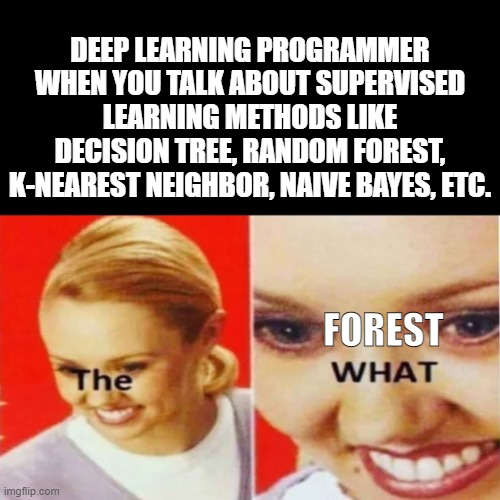
\includegraphics[width=0.5\textwidth]{figures/meme.jpg}
    \caption{ミーム.}
    \label{fig:appx:meme}
\end{figure*}

\chapter{\cref{ch:results} Details}\label{ch:appx:result-detail}
こんにちは Hogehoge, こんにちは Hogehoge, こんにちは Hogehoge, こんにちは Hogehoge, こんにちは Hogehoge, こんにちは Hogehoge, こんにちは Hogehoge, こんにちは Hogehoge, こんにちは Hogehoge, こんにちは Hogehoge, こんにちは Hogehoge, こんにちは Hogehoge, こんにちは Hogehoge, こんにちは Hogehoge, こんにちは Hogehoge, こんにちは Hogehoge, こんにちは Hogehoge, こんにちは Hogehoge, こんにちは Hogehoge
\begin{table}[h]
\centering
\begin{tabular}{|c|c|}\hline
    \textbf{Animal} & \textbf{Sound} \\\hline
    Cow & Moo \\\hline
    Sheep & Baa \\\hline
    Cat & Meow \\\hline
    Dog & Woof \\\hline
    Chicken & Cluck \\\hline
\end{tabular}
\caption{Animal sounds}
\label{tab:appx:animal-sound}
\end{table}